\documentclass[a4paper,11pt]{article}
\usepackage[utf8]{inputenc}
\usepackage[T1]{fontenc}
\usepackage[frenchb]{babel}

%%% INTERLIGNE
\usepackage{setspace}
\onehalfspacing
%\doublespacing

%%% PAGE DIMENSIONS
\usepackage{geometry} % to change the page dimensions
\geometry{a4paper} % or letterpaper (US) or a5paper or....
\geometry{margin=2.5cm} % for example, change the margins to 2 inches all round
% \geometry{landscape} % set up the page for landscape
% read geometry.pdf for detailed page layout information

%%% IMAGES ET FIGURES
\usepackage{graphicx}
%\usepackage{wrapfig}
\usepackage{float}

%opening
\title{Projet de Modal Image : Détection automatique des faces d'un RubiksCube}
\author{Cédric \bsc{Dessez}}
\date{29 juin 2012}

%%% PACKAGES
\usepackage{booktabs} % for much better looking tables
\usepackage{array} % for better arrays (erag matrices) in maths
\usepackage{paralist} % very flexible & customisable lists
% (eg. enumerate/itemize, etc.)
\usepackage{verbatim} % adds environment for commenting out blocks of
% text & for better verbatim
\usepackage{subfig} % make it possible to include more than one
% captioned figure/table in a single float These packages are all
% incorporated in the memoir class to one degree or another...
\usepackage{amsmath}

\begin{document}

\maketitle

\begin{figure}[h]
\begin{center}
 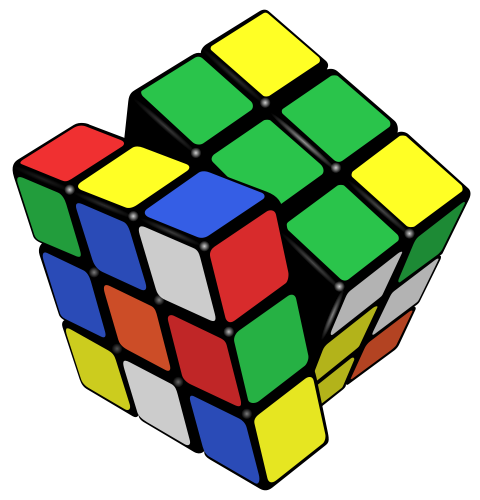
\includegraphics[width=10cm]{garde.png} 
\end{center}
\end{figure}
%\begin{abstract}
%\end{abstract}

\newpage
\tableofcontents
\newpage

%%%%%%%%%%%%%%%%%%%%%%%%%%%%%%%%%%%%%%%%%%%%%%%%%%%%%%%%%%%%%%%%%%%%%%%%%%%%%%%%%%%%%%%%%%%%%%%%%%%%%%%%%%%%%%
%%%%%%%%%%%%%%%%%%%%%%%%%%%%%%%%%%%%%%%%%%%%%%%%%%%%%%%%%%%%%%%%%%%%%%%%%%%%%%%%%%%%%%%%%%%%%%%%%%%%%%%%%%%%%%
\section{Introduction}
Le RubiksCube est un objet indémodable qui a poussé de nombreuses personnes à implémenter des algorithmes 
permettant de le résoudre, en essayant parfois de trouver le plus rapide. On peut imaginer que ce type de 
programme permette à des novices de reformer la forme résolue du Cube simplement en suivant des instructions
que lui fournit le programme.
Mais avant de lancer un tel algorithme, il faut lui indiquer la configuration initiale.
Certains de ces programmes sont peu ergonomiques et récupèrent l'information comme une suite formatée de 
caractères, d'autres le sont un peu plus et intègrent une interface graphique permettant de choisir les couleurs des
facettes en cliquant sur une représentation 3D. Mais il reste toujours long et fastidieux de devoir renseigner
une à une les couleurs des 54 facettes. D'où l'idée de réaliser un programme utilisant la webcam qui détecterait
la configuration lorsque l'utilisateur lui montre les faces les unes après les autres. Cela serait alors beaucoup
plus rapide et agréable.

Le cahier des charges de ce projet est donc le suivant : la solution implémentée doit détecter une face du 
RubiksCube qui est montrée à la webcam et l'enregistrer si elle s'est stabilisée. Dans ce cas elle est affichée
sur un patron de RubiksCube ce qui indique à l'utilisateur qu'il peut montrer la face suivante. La seule
contrainte est qu'il doit montrer ces faces dans le bon ordre selon un scénario prévu à l'avance. En effet, 
détecter le 
mouvement des faces pour en déduire quelle est la face que nous montre l'utilisateur compliquerait énormément 
la tâche.

%%%%%%%%%%%%%%%%%%%%%%%%%%%%%%%%%%%%%%%%%%%%%%%%%%%%%%%%%%%%%%%%%%%%%%%%%%%%%%%%%%%%%%%%%%%%%%%%%%%%%%%%%%%%%%
%%%%%%%%%%%%%%%%%%%%%%%%%%%%%%%%%%%%%%%%%%%%%%%%%%%%%%%%%%%%%%%%%%%%%%%%%%%%%%%%%%%%%%%%%%%%%%%%%%%%%%%%%%%%%%
\section{Principe générale de l'algorithme}
La solution implémentée repose sur la détection des facettes du RubiksCube par leurs couleurs qui sont assez
particulières et distinctes pour être discriminées les unes par rapport aux autres et pour être reconnues au 
sein d'une image capturée par la webcam. La première étape est donc d'extraire pour chacune des six couleurs
les zones qui s'en rapprochent le plus.

Puis il faut reconnaître et sélectionner les tâches de couleur qui forment les facettes de la face à détecter.
Cela se fait en deux étapes. La première consiste en un premier tri qui considère chaque composante connexe une 
à une dans les surfaces extraites à l'étape précédente, et qui la conserve ou non suivant des critères géométriques.
Puis, une deuxième étape consiste à détecter des alignements de trois composantes alignées, ce qui permet de 
trouver les bonnes et de les caractériser.

A partir de l'ensemble de ces éléments et des caractéristiques qui leur sont associées, l'étape suivante permet
d'associer à chacune d'entre eux un emplacement dans la matrice $3\times3$ représentant la face du Cube, 
construisant ainsi sa structure.

A ce stade, nous sommes donc capables de traiter indépendamment chaque image envoyée par la webcam pour y 
détecter ou non une face. Il nous faut dès lors détecter lorsque l'image se stabilise et lorsque l'on doit 
passer à la face suivante. Il s'agit donc de gérer temporellement la succession des images et le scénario 
d'exécution.

%%%%%%%%%%%%%%%%%%%%%%%%%%%%%%%%%%%%%%%%%%%%%%%%%%%%%%%%%%%%%%%%%%%%%%%%%%%%%%%%%%%%%%%%%%%%%%%%%%%%%%%%%%%%%%
%%%%%%%%%%%%%%%%%%%%%%%%%%%%%%%%%%%%%%%%%%%%%%%%%%%%%%%%%%%%%%%%%%%%%%%%%%%%%%%%%%%%%%%%%%%%%%%%%%%%%%%%%%%%%%
\section{Détail des différentes étapes}

%%%%%%%%%%%%%%%%%%%%%%%%%%%%%%%%%%%%%%%%%%%%%%%%%%%%%%%%%%%%%%%%%%%%%%%%%%%%%%%%%%%%%%%%%%%%%%%%%%%%%%%%%%%%%%
\subsection{Reconnaissance des 6 couleurs}
La reconnaissance des 6 couleurs du RubiksCube est une étape cruciale de la détection. En effet, c'est le biais
par lequel on passe d'une image brute en sortie de webcam à un premier stade d'information. Notons que pour
détecter l'emplacement du Cube, on aurait pu tenter de détecter les segments noirs qui délimitent les faces et
qui forment une sorte de quadrillage. Cependant, la détection de droite aurait certainement conduit à beaucoup
trop d'outliers et aurait été facilement perturbée par un arrière-plan un peu trop géométrique.

\subparagraph{L'espace de couleur HSV} 
Certes, les six couleurs du RubiksCube sont assez distinctes et discriminables, mais il est important de passer
dans le bon espace de couleur pour réaliser la segmentation de couleurs. En effet, il est important pour nous
qu'elle se fasse autant que faire se peut sans être trop influencée par la luminosité variable de l'image.
Ainsi, j'ai choisi de passer en représentation HSV (Hue Saturation Value) et de me baser principalement,
au moins pour 5 des 6 couleurs, sur la composante de teinte H. 

Ces cinq couleurs sont le rouge, le vert, le bleu, le orange et le jaune. J'extrais celles-ci en ne conservant
que les pixels dont la composante H se situe dans un certain intervalle autour de leur valeur typique. J'écarte
de plus ceux pour lesquels les valeurs de S et V sont inférieures à certains seuils pour lesquels la valeur de 
H perd grandement de sa pertinence (couleurs trop sombres ou trop peu saturées). Les valeurs des bornes des
intervalles et des seuils sont optimisées empiriquement à la main pour chaque couleur.

Le blanc, quand à lui est par définition une couleur absente du cercle de teintes qui se caractérise par une 
saturation maximale et une forte luminosité. De ce fait, la segmentation du blanc correspond à des seuils sur
les composantes S et V.

Notons que l'on apporte un soin particulier à obtenir des ensembles de couleurs qui sont disjoints, afin de
ne pas détecter deux facettes de couleurs différentes au même endroit !

\subparagraph{Lissage}
Le problème de cette segmentation est qu'elle nous donne une image assez bruitée. On applique donc deux filtres
d'opening qui vont permettre d'éliminer les points isolés et de lisser les contours.

On obtient alors 6 images binaires représentant les surfaces de l'image sur lesquelles se trouvent
les facettes du Cube (voir figure 1).

\begin{figure}[h]
\begin{center}
 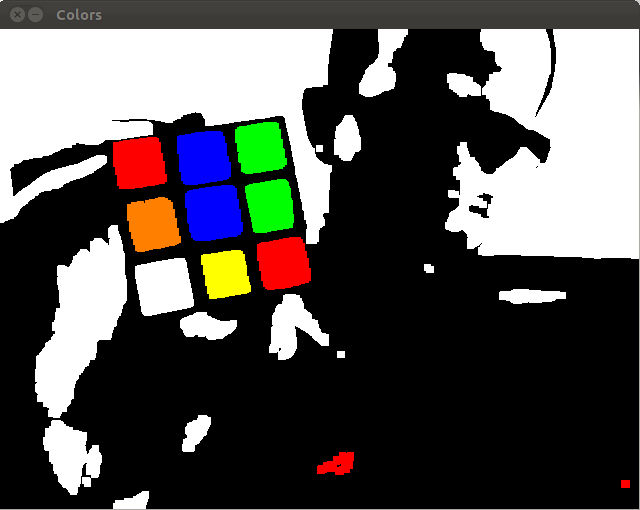
\includegraphics[width=10cm]{couleurs.png} 
\end{center}
 \caption{Extraction de couleurs}
 \label{Extraction de couleurs}
\end{figure}

\subparagraph{Problèmes liés à la segmentation de couleurs}
Le principal problème rencontré quant à la détection de couleurs est la présence de reflets sur les faces. En
effet les autocollants de couleur sont en plastique lisse et réfléchissent donc très bien la lumière. De ce fait, on
est obligé de montrer le cube sous un angle favorable pour éviter les reflets. Cela limite l'ergonomie du 
programme mais on ne peut pas y faire grand chose, si ce n'est éviter d'être face à une source de lumière trop
forte.

%%%%%%%%%%%%%%%%%%%%%%%%%%%%%%%%%%%%%%%%%%%%%%%%%%%%%%%%%%%%%%%%%%%%%%%%%%%%%%%%%%%%%%%%%%%%%%%%%%%%%%%%%%%%%%
\subsection{Extraction et sélection des composantes connexes}
Une fois les 6 images de couleurs extraites, on extrait les composantes connexes de chacune d'entre elles par
le biais de la fonction \verb|findContours| d'OpenCV que l'on applique successivement sur chacune d'elles.
Les contours renvoyés par cette fonction sont des objets \verb|vector<Point>|.

Simultanément à cette détection de contours, on réalise une première sélection sur chacun d'eux indépendamment
les uns des autres, et en se basant sur des critères géométriques simples.

Un premier filtre à ce stade consiste à éliminer les contours dont la taille est soit trop petite, soit trop
grande (les seuils correspondants utilisés pour le périmètre sont $100$ et $250$ pixels).

\begin{figure}[ht]
\begin{center}
 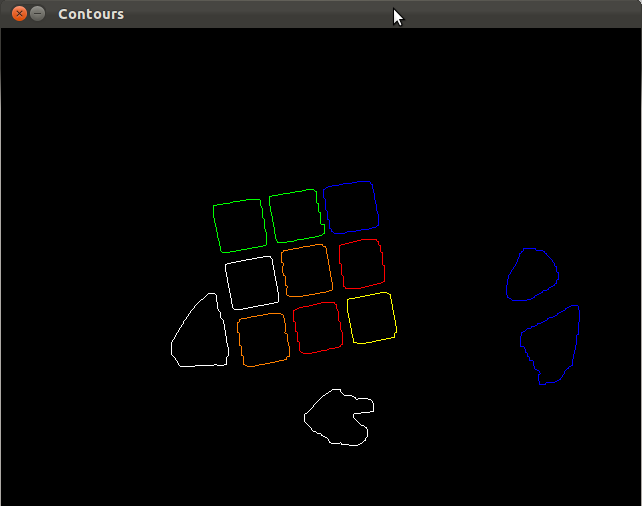
\includegraphics[width=10cm]{contours.png} 
\end{center}
 \caption{Sélection des contours}
 \label{Sélection des contours}
\end{figure}

Le second filtre est un peu plus poussé et nécessite dans un premier temps de déterminer le rectangle de surface
minimale englobant le contour traité à l'aide de la fonction \verb|minAreaRect| d'OpenCV. 
On vérifie alors que le rapport $longueur / largeur$ est proche de $1$.
Si ce n'était pas le cas, ce contour aurait peu de chance d'être une facette carrée de RubiksCube. Ainsi, on
écarte les contours pour lesquels ce rapport est compris entre $0,75$ et $1,33$.

Pour enregistrer les contours ayant passé ces deux premiers filtres, on souhaite caractériser chacun d'entre eux
non seulement par le tracé de son contours, mais aussi par une couleur suivant l'image dans laquelle on l'a 
trouvé. D'où l'implémentation d'une classe \verb|Contour| qui hérite de \verb|vector<Point>| et qui possède
des attributs supplémentaires, et notamment un champs \verb|color|, un champs \verb|center| de type \verb|Point|,
et un champs \verb|width|. Ces deux derniers champs résultent du calcul du rectangle englobant et trouveront
leur intérêt dans l'étape de sélection suivante.

Ces deux premiers filtres permettent d'éliminer une grande majorité des outliers mais ce n'est pas suffisant.
D'autant plus qu'on ne dispose pour chaque contours que de sa couleur et sa position géographique. Il est donc
nécessaire d'en savoir plus car même en supposant qu'après la présente étape on n'a plus que les 9 facettes que
l'on cherche, elles ne sont pas ordonnées et on ne saurait donc pas où les placer dans la matrice $3\times3$
représentant la face. C'est donc le but de l'étape suivante.

%%%%%%%%%%%%%%%%%%%%%%%%%%%%%%%%%%%%%%%%%%%%%%%%%%%%%%%%%%%%%%%%%%%%%%%%%%%%%%%%%%%%%%%%%%%%%%%%%%%%%%%%%%%%%%
\subsection{Sélection et caractérisation des facettes}
Cette nouvelle phase de sélection et caractérisation considère non plus les contours un par un mais trois par
trois. L'idée est de reconnaître des configurations géométriques simples de 3 contours, caractéristiques du 
schéma que l'on souhaite détecter. En effet, les facettes sont alignées trois par trois de manière régulière.
On prend donc deux contours parmi ceux renvoyés par la sélection précédente, et on cherche un troisième contour
qui est au milieu du segment formé par les deux premiers. On rajoute à cela des contraintes sur la cohérences 
des caractéristiques géométriques des triplets de contours et on incrémente des compteurs internes aux objets
de type \verb|Contour| afin d'indiquer pour chacun qu'il a été détecté dans une configuration valide, et de
préciser à quelle place dans cette configuration.

Voyons maintenant tout cela plus en détail.

On commence par prendre une paire d'objets \verb|Contour| dans le \verb|vector<Contour>| à notre 
disposition (on essaye toutes les paires possibles). Cette paire doit alors satisfaire deux premières 
contraintes : leurs tailles doivent être les mêmes (ce que l'on traduit par un intervalle admissible pour le 
rapport des deux côtés des facettes), et la distance entre leurs centres doit être inférieure à $2,7$ fois le 
côté d'une facette, ce qui
assure non seulement une sécurité supplémentaire permettant d'écarter certains outliers, mais qui permet aussi
de ne pas détecter les configurations diagonales où la facette centrale de la face se trouve au milieu de deux
coins opposés. Le nombre de paires qui remplissent ces critères et pour lesquelles on doit chercher un milieu 
est alors considérablement réduit, ce qui diminue la complexité de l'algorithme.

Puis, on cherche parmi tous les autres contours s'il y en a un de la même taille dont le centre se trouve environ
au milieu du segment reliant les centres des deux premiers.

Dans le cas où on arrive jusque là, le triplet de contours est considéré comme valide. La classe \verb|Contour| 
contient deux champs : \verb|isExt| et \verb|isInt| de type \verb|int| réalisant des compteurs. Pour un triplet
valide, on incrémente les compteurs \verb|isExt| des deux contours extérieurs, et le compteur \verb|isInt| du 
contour du milieu.

Un fois toutes les paires de contours testés, non seulement on ne garde que ceux pour lesquels les compteurs sont
non nuls, mais on est plus restrictif que cela : on n'accepte que ceux dont le couple $(isExt,isInt)$ a une des
valeurs suivantes :
\begin{itemize}
 \item $(0, 2)$ qui correspond à la facette centrale
 \item $(1, 1)$ qui correspond à une arrête
 \item $(2, 0)$ qui correspond à un coin.
\end{itemize}
De la sorte, on réduit encore un peu plus le risque de détecter des outliers et on classe les faces détectées en
trois catégories. C'est un premier pas vers la répartition des facettes dans la matrice $3\times3$ que l'on 
cherche à reconstituer.

%%%%%%%%%%%%%%%%%%%%%%%%%%%%%%%%%%%%%%%%%%%%%%%%%%%%%%%%%%%%%%%%%%%%%%%%%%%%%%%%%%%%%%%%%%%%%%%%%%%%%%%%%%%%%%
\subsection{Extraction de la structure d'une face du RubiksCube}
C'est finalement dans cette étape que l'on reconstitue vraiment la face du cube.

Pour représenter le résultat, j'ai implémenté une classe \verb|RubiksFace| dont l'unique attribut est une matrice
\verb|int cases[3][3]| telle que chaque case contient le code de la couleur de la facette correspondante. Cette
classe implémente des accesseurs simples à ces cases, et l'opérateur d'égalité \verb|==| entre deux objets
\verb|RubiksFace|.

C'est dans cette étape que l'on peut faire échouer la détection, si les conditions ne sont pas réunies pour 
extraire une structure de RubiksFace convenable.

On commence par construire trois objets de type \verb|vector<Contour*>| : \verb|centers|, \verb|edges| et 
\verb|corners| dans lequel on trie les contours selon les trois catégories décrites précédemment.
Alors la première cause d'échec est que ces vecteurs ne contiennent pas le bon nombre d'éléments. Si les 
contours renvoyés par l'étape précédente sont bien ceux d'une face de RubiksCube, il doit y avoir 1 élément
dans \verb|centers|, et 4 éléments dans \verb|edges| et dans \verb|corners|.

Néanmoins, on s'autorise à être un peu plus souple pour \verb|centers| en permettant jusqu'à 2 éléments 
en raison du motif dessiné sur la facette
centrale blanche du Cube, qui peut induire un contour supplémentaire. Dans ce cas, on exige néanmoins que ces
deux contours aient la même couleur.

Reste alors à répartir les contours de \verb|edges| et de \verb|corners| dans les cases correspondantes. Pour cela,
on utilise les coordonnées des centres des quatre éléments. Pour les arrêtes (\verb|edges|), on met dans la case
du haut celle dont l'ordonnée \verb|center.y| est minimale, en bas celle dont elle est maximale. On met dans 
la case de gauche celle dont l'abscisse \verb|center.x| est minimale et dans la case de droite celle dont elle 
est maximale.

On utilise le même procédé pour répartir les éléments de \verb|corners| dans la matrice de l'instance de 
\verb|RubiksFace|, mais on a besoin pour cela d'utiliser non plus les coordonnées du centre, mais les combinaisons
linéaires suivantes (on tourne le repère de 45\textdegree) :
\begin{center}
 \verb|center.x - center.y  | et \verb|  center.x + center.y| .
\end{center}

Cette étape était la dernière du traitement image par image du flux vidéo. La fonction correspondante renvoie
un booléen indiquant si la détection a réussi, et si tel est le cas, modifie l'objet \verb|RubiksFace| passé par 
référence.

\begin{figure}[h]
\begin{center}
 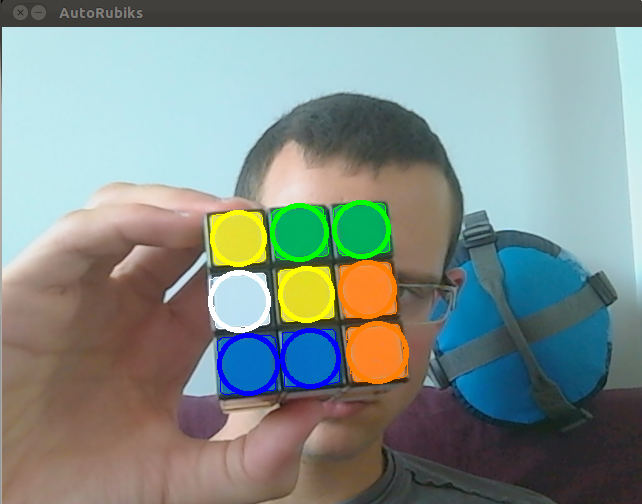
\includegraphics[width=10cm]{webcam.png} 
\end{center}
 \caption{Affichage de la détection}
 \label{Affichage de la détection}
\end{figure}

%%%%%%%%%%%%%%%%%%%%%%%%%%%%%%%%%%%%%%%%%%%%%%%%%%%%%%%%%%%%%%%%%%%%%%%%%%%%%%%%%%%%%%%%%%%%%%%%%%%%%%%%%%%%%%
\subsection{Gestion temporelle de la détection - Scénario}
Rappelons le scénario prévu initialement dans le cahier des charges. L'utilisateur doit présenter successivement
les 6 faces du Cube dans l'ordre suivant : il faut tourner le Cube comme si on le déroulait sur le patron de la
figure 4 de gauche à droite puis la face du haut, puis celle du bas.

\begin{figure}[h]
\begin{center}
 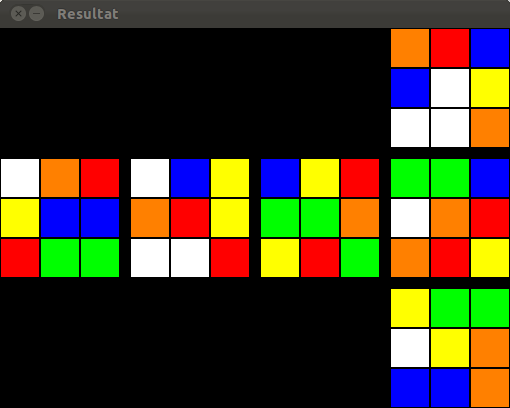
\includegraphics[width=8cm]{patron.png} 
\end{center}
 \caption{Patron du RubiksCube}
 \label{Patron du RubiksCube}
\end{figure}

Pour gérer la succession des faces, les enregistrer et afficher le patron en train de se remplir, j'ai implémenté
la classe \verb|Rubiks| qui comprend juste un constructeur et la méthode \verb|setNewFace(const| 
\verb|RubiksFace& face)|, 
et qui encapsule un tableau de 6 objets \verb|RubiksFace| et l'image du patron.

Le passage d'une face à l'autre se fait lorsque la détection s'est stabilisée. Détaillons ce que l'on entend
par stabilisation. Il faut que la même face ait été détectée 10 fois sans qu'aucune autre n'ait été détectée 
entre temps. Pour cela, on garde en mémoire un compteur et la \verb|RubiksFace| courante. Lorsqu'on détecte une
face différente de cette dernière, on réinitialise le compteur à 1 et on l'actualise. Si on détecte la même face
que celle enregistrée, on incrémente le compteur. Enfin, si la détection échoue, on ne fait rien. A chaque fois
que la détection réussit, on teste la valeur du compteur et s'il vaut 10, on appelle la méthode 
\verb|setNewFace|. L'utilisateur sait qu'il peut passer à la face suivante car il voit s'afficher la face
détectée sur le patron.

Notons que l'on ne demande pas à avoir un certain nombre de frames successives du flux vidéo avec la même face
détectée car la détection n'est pas suffisamment stable et le bruit induit parfois un clignotement qui
pourrait rendre la détection très compliquée voir impossible.

Une fois la dernière face détectée, le programme se fige et on pourrait envoyer la configuration du RubiksCube
à un programme de résolution.

%%%%%%%%%%%%%%%%%%%%%%%%%%%%%%%%%%%%%%%%%%%%%%%%%%%%%%%%%%%%%%%%%%%%%%%%%%%%%%%%%%%%%%%%%%%%%%%%%%%%%%%%%%%%%%
%%%%%%%%%%%%%%%%%%%%%%%%%%%%%%%%%%%%%%%%%%%%%%%%%%%%%%%%%%%%%%%%%%%%%%%%%%%%%%%%%%%%%%%%%%%%%%%%%%%%%%%%%%%%%%
\section{Analyse de la performance, perspectives d'évolution}
Le programme fonctionne plutôt bien de manière générale mais quelques problèmes persistent. La majorité d'entre
eux interviennent dès la première étape de la détection du Cube, au niveau de la détection de couleurs.

\subsection{Reflets lumineux} 
Ce problème a déjà été évoqué précédemment. Les facettes sont des autocollants en plastique lisse qui ont un
effet miroir particulièrement important qui empêche parfois la détection des faces ou en change la couleur.
Ainsi, l'utilisateur doit légèrement incliner le Cube sous un angle favorable afin d'éviter tout reflet, ce
qui réduit un peu l'ergonomie. Cependant, on ne peut rien faire pour éviter ça (on ne va quand même pas poncer
les facettes du RubiksCube !), si ce n'est éviter de se placer face à des sources de lumières lors de l'exécution
(l'écran ayant parfois le mauvais goût d'être lui-même un source de lumière intense si la luminosité est basse !).

\subparagraph{Mauvaise adaptation à l'éclairage ambiant}
On remarque que l'image délivrée par la webcam subit un réglage automatique de l'ordinateur qui tend à optimiser
la luminosité et le contraste. Ce réglage automatique nous rend bien service puisqu'il nous évite de le faire 
nous-même. Cependant, dans des cas trop extrêmes de forte ou faible luminosité ambiante ou d'éclairage 
légèrement coloré, la détection de nos 6 couleurs est altérée et n'est plus efficace.

Une solution à ce problème pourrait être d'implémenter soi-même le réglage automatique, ou bien de calibrer les 
couleurs une à une avant la détection en demandant à l'utilisateur de les montrer à la webcam. Une autre solution
bien plus technique serait de réimplémenter nous-même le réglage automatique de la webcam.

\subparagraph{Détection du mouvement du RubiksCube}
Afin de rendre le programme encore plus ergonomique, il faudrait que l'utilisateur n'ait pas besoin de respecter
le bon ordre des faces mais qu'il puisse simplement les montrer au hasard et que le programme détecte le 
mouvement du Cube afin de déterminer la bonne. 

Les algorithmes mis en place seraient alors susceptibles d'implémenter une souris 3D à l'aide du RubiksCube,
ce qui était une des idées de projets envisagées pour ce modal.

Cependant, la détection prend une autre dimension et demande une implémentation beaucoup plus subtile et poussée
que je n'avais pas le temps de faire, même ayant fini l'implémentation de mon programme une séance en avance.

\paragraph{  }
C'est ainsi que pour occuper ma dernière séance de modal, j'ai implémenté un programme différent, mais qui
utilise le travail déjà réalisé de détection du Cube.

%%%%%%%%%%%%%%%%%%%%%%%%%%%%%%%%%%%%%%%%%%%%%%%%%%%%%%%%%%%%%%%%%%%%%%%%%%%%%%%%%%%%%%%%%%%%%%%%%%%%%%%%%%%%%%
%%%%%%%%%%%%%%%%%%%%%%%%%%%%%%%%%%%%%%%%%%%%%%%%%%%%%%%%%%%%%%%%%%%%%%%%%%%%%%%%%%%%%%%%%%%%%%%%%%%%%%%%%%%%%%
\section{Réalisation Annexe : image superposée à une face du cube}
Avec le temps qui me restait une fois le programme de détection fini, j'ai voulu réutiliser le travail de 
détection réalisé pour réaliser un programme qui remplace à l'écran la face du RubiksCube par une image définie
à l'avance.

\begin{figure}[h]
\begin{center}
 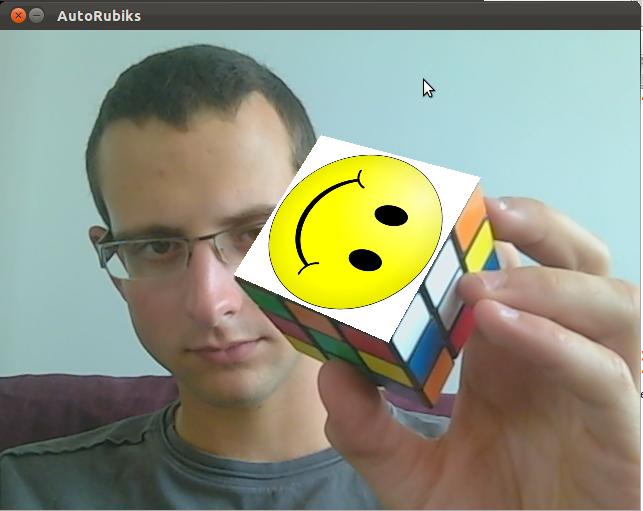
\includegraphics[width=10cm]{smiley.png} 
\end{center}
 \caption{Projection d'image}
 \label{Projection d'image}
\end{figure}

L'utilité d'un tel programme (ou le RubiksCube serait remplacé par autre chose, une tablette par exemple)
pourrait être par exemple d'afficher en temps réel une publicité sur un flux d'image et ainsi économiser une
impression papier.

Un première étape de l'exécution de ce programme consiste à appuyer sur une touche ('a' en l'occurrence) pour
indiquer au programme que la face qu'on lui montre est celle sur laquelle on veut superposer l'image. Dès lors,
à chaque
fois que le programme détecte une face, si c'est la même que celle qu'on a indiqué, alors l'image prédéfini
s'y superpose.

Cette superposition se fait par une homographie appliquée avec la fonction \verb|warpPerspective|. Cependant,
il faut au préalable calculer cette homographie. Pour cela, on utilise la fonction \verb|findHomography| en lui
fournissant 9 points : ceux des centres des facettes, et les 9 points correspondants dans l'image à intégrer.
Quatre points auraient été suffisants mais la précision est accrue lorsque l'on en fournit plus. L'extrapolation
est alors bien meilleure et on obtient une image très stable qui ne tremble pas.

Cependant, notons qu'une face enregistrée par un objet \verb|RubiksFace| enregistre non seulement la face mais aussi 
son orientation (4 orientations possibles tous les quarts de tour). De ce fait, détecter que la face est ou
non la même que cette indiquée par l'utilisateur nécessite de tester les 4 orientations possibles. Cela permet
aussi de pouvoir tourner la face comme on le souhaite : l'image superposée tourne aussi. 

Afin de rendre cette détection possible en temps réel, la classe \verb|RubiksFace| ne stocke non plus des \verb|int|
codant simplement une couleur, mais des instances d'une nouvelle classe \verb|Facette| qui stocke la couleur et
les coordonnées du centre. On aurait pu stocker des objets \verb|Contour| mais cela aurait été très lourd car
on aurait traîné inutilement les coordonnées de tous les points composant le contour détecté de la facette.

La classe \verb|RubiksFace| encapsule également toutes les fonctions implémentant les tests d'égalité et les 
rotations effectuées.

Ce programme annexe marche relativement bien, même si la méthode de détection du Cube réutilisée n'est pas
idéale car beaucoup trop restrictive et exigente. Le problème est que la détection en elle-même n'est pas suffisamment
stable, et ainsi l'image a tendance à clignoter.

%%%%%%%%%%%%%%%%%%%%%%%%%%%%%%%%%%%%%%%%%%%%%%%%%%%%%%%%%%%%%%%%%%%%%%%%%%%%%%%%%%%%%%%%%%%%%%%%%%%%%%%%%%%%%%
%%%%%%%%%%%%%%%%%%%%%%%%%%%%%%%%%%%%%%%%%%%%%%%%%%%%%%%%%%%%%%%%%%%%%%%%%%%%%%%%%%%%%%%%%%%%%%%%%%%%%%%%%%%%%%
\section{Remerciements}
Je tiens à remercier M. Renaud Keriven pour l'aide et le soutien qu'il nous a apporté tout au long de ces neuf
séances, ainsi que pour les connaissances acquises pendant ce modal.

Je souhaite enfin à remercier non seulement M. Keriven, mais aussi mes camarades du groupe de modal pour la 
bonne humeur et la bonne ambiance dans laquelle s'est déroulée ce module.



\end{document}
